\clearpage
\begingroup
\let\clearpage\relax
\let\cleardoublepage\relax
\vspace*{\fill}
\chapter{网络层：控制平面}
\begin{center}
控制平面回答「路由表怎么算出来」。本章讲链路状态与距离向量两类路由算法，以及 OSPF、BGP、ICMP 与 SDN 的角色。
\end{center}
\vspace*{\fill}
\endgroup
\clearpage

\section{路由算法：动机与分类}

上一章的数据平面解决「一个到达的分组从哪个端口出去」，它依赖路由器中已存在的\textbf{转发表}。但转发表并非凭空产生：路由器如何知道去往某个目的网络应当把分组交给哪个邻居？这属于\textbf{控制平面}的任务。控制平面的核心是一个\textbf{路由算法 (routing algorithm)}：给定全网链路代价，求从源到目的地的「最小代价路径」。

\subsection{代价模型}

把网络抽象为带权无向图 $G=(V,E)$，$V$ 是路由器（或子网）集合，$E$ 是链路集合。对每条链路 $(x,y)\in E$ 定义一个非负代价
\begin{equation}
    c(x,y) > 0, \qquad c(x,y)=c(y,x),
\end{equation}
并约定若 $x$ 与 $y$ 不相邻则 $c(x,y)=\infty$。代价可以是物理量，也可以是策略量：
\begin{itemize}
    \item \textbf{跳数 (hop count)}：$c\equiv 1$，即最少中转次数；
    \item \textbf{带宽的倒数}：$\sim 1/B$，鼓励走高速链路；
    \item \textbf{时延、拥塞或可靠性}：把排队时延、丢包率折算为代价；
    \item \textbf{策略权重}：管理员人为设定的偏好（如「不走便宜但不靠谱的链路」）。
\end{itemize}

一条路径 $P=(x_0,x_1,\dots,x_k)$ 的代价是各段之和
\begin{equation}
    c(P) = \sum_{i=1}^{k} c(x_{i-1},x_i),
\end{equation}
\textbf{最小代价路径}就是使 $c(P)$ 取最小的路径；当所有代价满足 $c(x,y)>0$ 时，最短路构成一棵以源为根的\textbf{最短路树 (shortest-path tree)}。

\subsection{两类路由算法}

按「谁来收集全局信息、如何计算」划分：

\begin{itemize}
    \item \textbf{集中式 (centralized) 算法}：某处（逻辑上）掌握完整拓扑与全部链路代价，再一次性算出所有最短路。这类算法又称\textbf{链路状态 (Link State, LS)}算法，因为前提是每个节点都能得到全网链路状态。
    \item \textbf{分布式 (decentralized) 算法}：没有全局视图。每个节点只知道自己到邻居的代价，通过与邻居迭代交换信息，逐步逼近最短路。代表是\textbf{距离向量 (Distance Vector, DV)}算法。
\end{itemize}

\begin{table}[H]
\centering
\caption{链路状态与距离向量的对比}
\renewcommand{\arraystretch}{1.4}
\begin{tabulary}{\textwidth}{@{}CCC@{}}
\toprule
\textbf{维度} & \textbf{链路状态 (LS)} & \textbf{距离向量 (DV)} \\
\midrule
全局视图 & 需要，每节点同一张图 & 不需要，仅邻居距离 \\
信息交换 & 泛洪本节点链路状态 & 与邻居交换距离向量 \\
核心算法 & Dijkstra & Bellman--Ford 迭代 \\
收敛速度 & 较快 & 可能慢（计数到无穷） \\
典型协议 & OSPF、IS-IS & RIP \\
\bottomrule
\end{tabulary}
\end{table}

\section{链路状态路由算法：Dijkstra}

\subsection{机制}

链路状态算法的分工是「先让所有人看到同一张地图，再各自算最短路」：

\begin{enumerate}
    \item 每个节点周期性探测邻居，得到本节点的链路状态（邻居身份 + 代价）；
    \item 用\textbf{泛洪 (flooding)} 把链路状态分组 (Link State Packet, LSP) 发给全网；每个节点把收到的 LSP 汇总，重建出一张与所有节点一致的拓扑图 $G=(V,E)$；
    \item 每个节点在本地对 $G$ 运行 \textbf{Dijkstra 算法}，以自身为源求出到所有目的地的最短路径及下一跳，写入转发表。
\end{enumerate}

\subsection{算法}

Dijkstra 维护「已确定最短路的节点集合 $N'$」和「当前源到各节点的距离估计 $D(v)$」。每轮从未确定集合中挑出 $D$ 最小者加入 $N'$，并用它松弛其邻居。

\begin{algorithm}[H]
\caption{链路状态 Dijkstra 最短路}
\begin{algorithmic}[1]
\Procedure{LS-Dijkstra}{$s$}
    \State $N' \gets \{s\}$ \Comment{已确定最短路的节点集合}
    \ForAll{节点 $v$}
        \If{$v$ 是 $s$ 的邻居} $D(v)\gets c(s,v)$ \Else $D(v)\gets\infty$ \EndIf
    \EndFor
    \While{$N' \ne V$}
        \State 取 $w \notin N'$ 使 $D(w)$ 最小 \Comment{不在 $N'$ 中距离最小的节点}
        \State $N' \gets N' \cup \{w\}$
        \ForAll{$w$ 的邻居 $v \notin N'$}
            \State $D(v) \gets \min\bigl(D(v),\, D(w)+c(w,v)\bigr)$ \Comment{松弛}
        \EndFor
    \EndWhile
\EndProcedure
\end{algorithmic}
\end{algorithm}

\subsection{六节点算例}

考虑经典拓扑（Kurose 的 $u,v,w,x,y,z$），链路代价标在图上。

\begin{figure}[H]
\centering
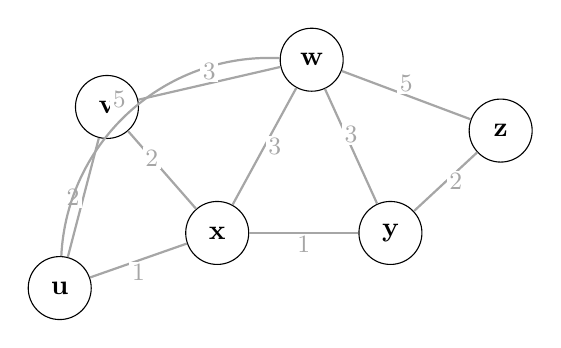
\begin{tikzpicture}[
    node/.style={circle, draw, minimum size=0.8cm, font=\bfseries},
    lbl/.style={font=\small, fill=white, inner sep=1pt},
    edge/.style={thick, gray!70}
]
    \node[node] (u) at (0,0)   {u};
    \node[node] (v) at (0.6,2.3) {v};
    \node[node] (w) at (3.2,2.9) {w};
    \node[node] (x) at (2.0,0.7) {x};
    \node[node] (y) at (4.2,0.7) {y};
    \node[node] (z) at (5.6,2.0) {z};

    \draw[edge] (u) -- node[lbl,left]{2} (v);
    \draw[edge] (u) -- node[lbl,below]{1} (x);
    \draw[edge] (u) to[bend left=45] node[lbl,above left]{5} (w);
    \draw[edge] (v) -- node[lbl,above]{3} (w);
    \draw[edge] (v) -- node[lbl,above left]{2} (x);
    \draw[edge] (w) -- node[lbl,right]{3} (x);
    \draw[edge] (w) -- node[lbl,above]{3} (y);
    \draw[edge] (w) -- node[lbl,above]{5} (z);
    \draw[edge] (x) -- node[lbl,below]{1} (y);
    \draw[edge] (y) -- node[lbl,right]{2} (z);
\end{tikzpicture}
\caption{链路状态算例拓扑：$u$ 为源，边上数字为链路代价}
\label{fig:ls_topo}
\end{figure}

从 $u$ 出发逐步执行，每轮选出一个节点加入 $N'$。表中 $D(\cdot)$ 写成「距离,前驱」的形式，\textbf{粗体}为该轮被选中的节点。

\begin{table}[H]
\centering
\caption{Dijkstra 从 $u$ 出发的逐步迭代表}
\renewcommand{\arraystretch}{1.35}
\small
\begin{tabulary}{\textwidth}{@{}c|C|C|C|C|C|C@{}}
\toprule
\textbf{轮} & \textbf{$N'$} & \textbf{$D(v)$} & \textbf{$D(w)$} & \textbf{$D(x)$} & \textbf{$D(y)$} & \textbf{$D(z)$} \\
\midrule
0 & $\{u\}$        & $2,u$ & $5,u$ & $\mathbf{1,u}$ & $\infty$ & $\infty$ \\
1 & $\{u,x\}$      & $2,u$ & $4,x$ & $1,u$          & $2,x$    & $\infty$ \\
2 & $\{u,x,v\}$    & $\mathbf{2,u}$ & $4,x$ & $1,u$ & $2,x$ & $\infty$ \\
3 & $\{u,x,v,y\}$  & $2,u$ & $4,x$ & $1,u$ & $\mathbf{2,x}$ & $4,y$ \\
4 & $\{u,x,v,y,w\}$& $2,u$ & $\mathbf{4,x}$ & $1,u$ & $2,x$ & $4,y$ \\
5 & 全部节点       & $2,u$ & $4,x$ & $1,u$ & $2,x$ & $\mathbf{4,y}$ \\
\bottomrule
\end{tabulary}
\end{table}

逐轮要点：
\begin{itemize}
    \item 第 0 轮：$u$ 的直接邻居为 $v,w,x$，距离分别为 $2,5,1$；$x$ 最小。
    \item 第 1 轮：加入 $x$ 后松弛其邻居——$w$ 由 $5$ 降为 $1+3=4$（前驱改 $x$），$y$ 由 $\infty$ 变 $1+1=2$。
    \item 第 2 轮：$v$ 的距离 $2$ 最小（与 $y$ 并列，约定任选其一），加入 $v$；经 $v$ 到 $w$ 为 $2+3=5>4$，不更新。
    \item 第 3 轮：加入 $y$，经 $y$ 到 $z$ 得 $2+2=4$。
    \item 第 4 轮：加入 $w$，经 $w$ 到 $z$ 为 $4+5=9>4$，不更新。
    \item 第 5 轮：最后加入 $z$，收敛。
\end{itemize}

于是 $u$ 到各目的的最小代价与下一跳为：

\begin{center}
$v:2$（经 $v$），$x:1$（经 $x$），$y:2$（经 $x$），$w:4$（经 $x$），$z:4$（经 $x$ $\to$ $y$）。
\end{center}

对应的最短路树如下（粗实线为树边，即每条路径的下一跳关系）。

\begin{figure}[H]
\centering
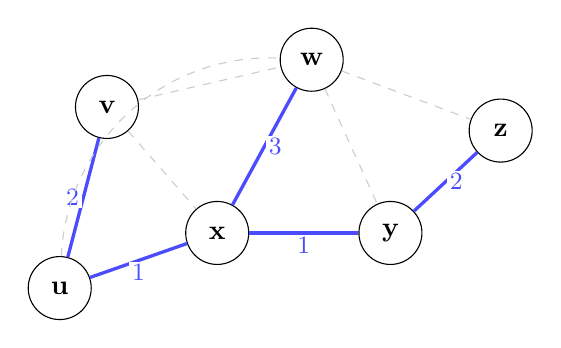
\begin{tikzpicture}[
    node/.style={circle, draw, minimum size=0.8cm, font=\bfseries},
    tree/.style={very thick, blue!70},
    lbl/.style={font=\small, fill=white, inner sep=1pt}
]
    \node[node] (u) at (0,0)   {u};
    \node[node] (v) at (0.6,2.3) {v};
    \node[node] (w) at (3.2,2.9) {w};
    \node[node] (x) at (2.0,0.7) {x};
    \node[node] (y) at (4.2,0.7) {y};
    \node[node] (z) at (5.6,2.0) {z};

    \draw[tree] (u) -- node[lbl,left]{2} (v);
    \draw[tree] (u) -- node[lbl,below]{1} (x);
    \draw[tree] (x) -- node[lbl,right]{3} (w);
    \draw[tree] (x) -- node[lbl,below]{1} (y);
    \draw[tree] (y) -- node[lbl,right]{2} (z);

    \draw[gray!40, dashed] (u) to[bend left=45] (w);
    \draw[gray!40, dashed] (v) -- (w);
    \draw[gray!40, dashed] (v) -- (x);
    \draw[gray!40, dashed] (w) -- (y);
    \draw[gray!40, dashed] (w) -- (z);
\end{tikzpicture}
\caption{以 $u$ 为根的最短路树：$u\to v$，$u\to x\to\{w,y\}$，$y\to z$}
\label{fig:ls_tree}
\end{figure}

\subsection{复杂度与讨论}

设 $|V|$ 个节点、$|E|$ 条链路。每轮需线性扫描未确定节点找最小 $D$，共 $|V|$ 轮，故朴素实现为
\begin{equation}
    T_{\text{naive}} = O\!\left(|V|^2\right).
\end{equation}
用二叉堆/斐波那契堆维护候选距离，可降为
\begin{equation}
    T_{\text{heap}} = O\!\left((|V|+|E|)\log|V|\right).
\end{equation}
LS 的代价是泛洪带来的开销 $O(|E|)$ 量级——每个节点都要把链路状态通告到全网。此外，若链路代价随负载动态变化，全网不同步地重算可能出现\textbf{路由振荡}：流量涌向「当前最便宜」的链路，反而把它压成最贵。缓解办法是让代价不直接正比于瞬时负载，或引入随机化。

\section{距离向量路由算法：Bellman--Ford}

\subsection{递推式与算法}

DV 算法基于动态规划：节点 $x$ 到目的 $y$ 的最短距离，等于「先花 $c(x,v)$ 走到某个邻居 $v$，再由 $v$ 走最短路到 $y$」在所有邻居中的最优值。这就是 \textbf{Bellman--Ford 方程}
\begin{equation}
    D_x(y) = \min_{v \in N(x)} \bigl\{\, c(x,v) + D_v(y) \,\bigr\},
    \label{eq:bf}
\end{equation}
其中 $N(x)$ 是 $x$ 的邻居集合。每个节点维护一个到全网各目的的距离向量 $D_x=[D_x(y)]_{y\in V}$，周期性或触发式地把自己的向量发给邻居。邻居拿到后用式 \eqref{eq:bf} 更新，若自身向量改变则继续通知其邻居。

\begin{algorithm}[H]
\caption{距离向量算法（在节点 $x$ 上运行）}
\begin{algorithmic}[1]
\Procedure{DV-Run}{$x$}
    \ForAll{目的 $y \in V$}
        \If{$y$ 是 $x$ 的邻居} $D_x(y)\gets c(x,y)$ \Else $D_x(y)\gets\infty$ \EndIf
    \EndFor
    \State 把向量 $D_x$ 发给所有邻居
    \Loop
        \State 等待：收到某邻居 $v$ 的向量 $D_v$，或本节点到某邻居的链路代价发生变化
        \ForAll{目的 $y \in V$}
            \State $D_x(y) \gets \min_{v\in N(x)} \bigl\{ c(x,v) + D_v(y) \bigr\}$ \Comment{按式 \eqref{eq:bf} 重算}
        \EndFor
        \If{$D_x$ 有任何分量改变} 把新向量 $D_x$ 发给所有邻居 \EndIf
    \EndLoop
\EndProcedure
\end{algorithmic}
\end{algorithm}

\subsection{好消息传得快}

当链路代价下降（好消息）时，DV 收敛很快。考虑简单的链 $x$--$y$--$z$，$c(x,y)=1$、$c(y,z)=1$。初始 $D_y(x)=1$，$D_z(x)=\infty$。若某时刻 $z$ 与 $x$ 直连的代价从 $\infty$ 降到 $2$：
\begin{itemize}
    \item $z$ 算出 $D_z(x)=\min(\infty,\,c(z,x)=2)=2$，通知 $y$；
    \item $y$ 算出 $D_y(x)=\min(c(y,z)+D_z(x),\,c(y,x),\,c(y,z)+D_z(x))=1+2=3$ 与直连 $1$ 比较取 $1$，其实不变；
    \item 若代价是\textbf{下降}（例如 $c(y,x)$ 由 $4$ 降到 $1$），$y$ 立即更新并把更小的 $D_y$ 广播出去，邻居再迅速改善。好消息一趟就能传遍，因为每一跳都在「下调」估计。
\end{itemize}

\subsection{坏消息传得慢：计数到无穷}

链路代价\textbf{上升}时情况截然不同。当节点发现经某邻居到达某目的地的路径其实绕回了自己，就会把错误的信息反复回传，估计值一轮一轮缓慢增大，称为\textbf{计数到无穷 (count to infinity)}。

取链 $x$--$y$--$z$，其中 $c(x,y)=4$、$c(y,z)=1$、$c(x,z)=50$。代价变化前达到的稳定态为
\begin{equation}
    D_y(x)=4 \;(\text{直连}), \qquad D_z(x)=\min(1+D_y(x),\,50)=5 \;(\text{经 }y).
\end{equation}
现在 $x$--$y$ 链路代价从 $4$ 骤升到 $60$（链路恶化）。$y$ 直接感知该变化，而 $z$ 尚未察觉。逐轮演算如下：

\begin{table}[H]
\centering
\caption{计数到无穷的逐步数值演算（$c(x,y):4\to 60$）}
\renewcommand{\arraystretch}{1.3}
\begin{tabulary}{\textwidth}{@{}c|C|C|L@{}}
\toprule
\textbf{轮次} & \textbf{$D_y(x)$} & \textbf{$D_z(x)$} & \textbf{说明} \\
\midrule
变化前 & $4$（直连） & $5$（经 $y$） & 稳定态 \\
1 & $6$（经 $z$） & $5$（经 $y$） & $y$: $\min(60,\,1+5)=6$ \\
2 & $6$ & $7$（经 $y$） & $z$: $\min(50,\,1+6)=7$ \\
3 & $8$（经 $z$） & $7$ & $y$: $\min(60,\,1+7)=8$ \\
4 & $8$ & $9$（经 $y$） & $z$: $\min(50,\,1+8)=9$ \\
5 & $10$（经 $z$） & $9$ & $y$: $\min(60,\,1+9)=10$ \\
$\vdots$ & $\vdots$ & $\vdots$ & 每轮各增 $2$，来回传播 \\
$k$ & $50$ & $49$ & $z$ 逼近其直连上限 $50$ \\
$k{+}1$ & $50$ & $50$ & $z$: $\min(50,\,1+50)=50$ \\
$k{+}2$ & $51$（经 $z$） & $50$ & 收敛：$y$ 走 $z$，$z$ 走直连 \\
\bottomrule
\end{tabulary}
\end{table}

要点：
\begin{itemize}
    \item $y$ 错误地以为「可以经 $z$ 到达 $x$」，而 $z$ 的路径恰恰又经过 $y$，形成\textbf{两节点路由环路}。
    \item 若 $x$--$z$ 之间根本不存在链路（$c(x,z)=\infty$），则 $D_y(x)$、$D_z(x)$ 会一直增大、永不收敛，这就是「计数到\emph{无穷}」的字面含义。
    \item 即使存在直连上限，收敛也要经历约 $(50-6)/2\approx 22$ 轮，期间分组可能在环中打转，响应极慢。
\end{itemize}

\subsection{缓解：水平分割与毒性逆转}

\textbf{水平分割 (split horizon)}：不把「到某目的地的距离」告诉通往该目的地的下一跳邻居，因为对方显然不该经由你到达该目的地。

\textbf{毒性逆转 (poisoned reverse)}：更强的版本——如果 $z$ 到 $x$ 的最短路是经 $y$ 的，那么 $z$ 通知 $y$ 时故意宣告 $D_z(x)=\infty$。在上例中，$z$ 会告诉 $y$「我无法到达 $x$」，于是 $y$ 不会误以为能经 $z$ 绕过去，两节点环路被立即切断。

毒性逆转并非万能：它只能消除两节点之间的环路，对于三节点及以上的环路仍可能失效。因此工程上常把 DV（如 RIP）限制在小规模网络，并配合较高的无穷大阈值、触发更新与抑制计时器。

\section{自治系统内部路由：OSPF}

现实互联网规模巨大，不可能让所有路由器运行同一个全局最短路。做法是把网络划分为若干\textbf{自治系统 (Autonomous System, AS)}，AS 内部使用\textbf{内部网关协议 (IGP)}，AS 之间使用\textbf{外部网关协议 (EGP)}。\textbf{OSPF (Open Shortest Path First)} 是应用最广的链路状态 IGP。

\subsection{机制与特性}

每个 OSPF 路由器泛洪链路状态通告，构建同一张拓扑图后运行 Dijkstra。相较朴素的 LS，OSPF 增加了多项工程能力：

\begin{itemize}
    \item \textbf{链路状态与 Dijkstra}：与前述链路状态算法原理一致，代价由管理员按带宽等设定。
    \item \textbf{分区域 (area)}：把 AS 再划分为若干区域以限制泛洪范围。一个特殊区域——\textbf{骨干区 (backbone area 0)}——连接所有其他区域。区域边界路由器 (ABR) 汇总区域间路由，自治系统边界路由器 (ASBR) 则与其他 AS 交换外部路由。分区域把链路状态通告的泛洪局部化，显著降低开销。
    \item \textbf{鉴别 (authentication)}：OSPF 报文可携带口令/MAC 鉴别，防止伪造的路由通告注入。
    \item \textbf{等代价多路径 (Equal-Cost Multi-Path, ECMP)}：当到同一目的存在多条等代价路径时，OSPF 可同时使用它们做负载分担，而非只保留一条。
    \item \textbf{快速收敛与可靠泛洪}：链路状态更新通过可靠机制传播，链路故障能被迅速检测并重新计算。
\end{itemize}

\begin{figure}[H]
\centering
\begin{tikzpicture}[
    rt/.style={circle, draw, minimum size=0.6cm, font=\small},
    abr/.style={circle, draw, fill=blue!15, minimum size=0.7cm, font=\small},
    lbl/.style={font=\small, align=center}
]
    \node[rt] (b1) at (0,0) {};
    \node[rt] (b2) at (1.4,0.6) {};
    \node[rt] (b3) at (1.4,-0.6) {};
    \node[abr] (ab1) at (3.0,0) {ABR};
    \draw (b1)--(b2); \draw (b1)--(b3); \draw (b2)--(ab1); \draw (b3)--(ab1);
    \node[lbl, above] at (1.0,0.9) {区域 0（骨干）};

    \node[rt] (a1) at (4.6,1.0) {};
    \node[rt] (a2) at (5.6,0.2) {};
    \node[rt] (a3) at (4.6,-1.0) {};
    \node[rt] (a4) at (5.6,-1.8) {};
    \draw (ab1)--(a1); \draw (a1)--(a2); \draw (ab1)--(a3); \draw (a3)--(a4); \draw (a2)--(a4);
    \node[lbl, align=center, anchor=west] at (6.1,-0.4) {区域 1\\(经 ABR 汇总)};

    \node[abr, fill=green!20] (asbr) at (-2.4,0) {ASBR};
    \draw (b1)--(asbr);
    \node[lbl, anchor=east] at (-2.9,0) {其他 AS};
\end{tikzpicture}
\caption{OSPF 层次结构：骨干区 0 汇聚各区域，ABR 汇总区域间路由，ASBR 连接外部 AS}
\label{fig:ospf_hier}
\end{figure}

OSPF 主要报文类型如下：

\begin{table}[H]
\centering
\caption{OSPF 五类报文}
\renewcommand{\arraystretch}{1.3}
\begin{tabulary}{\textwidth}{@{}CCL@{}}
\toprule
\textbf{类型} & \textbf{名称} & \textbf{用途} \\
\midrule
1 & Hello & 发现/维持邻居，选举指定路由器 \\
2 & Database Description & 交换链路状态数据库摘要 \\
3 & Link State Request & 请求缺失的链路状态通告 \\
4 & Link State Update & 泛洪链路状态通告（核心） \\
5 & Link State Ack & 确认收到通告，保证可靠泛洪 \\
\bottomrule
\end{tabulary}
\end{table}

\section{自治系统间路由：BGP}

AS 之间靠 \textbf{BGP (Border Gateway Protocol)} 交换可达性。与追求最短代价的 IGP 不同，BGP 的核心是\textbf{策略}：一个 AS 是否愿意为另一个 AS 转发流量，取决于商业关系（客户/提供商/对等），而非单纯的链路代价。因此 BGP 被称为互联网的「粘合剂」。

\subsection{路径向量与环路检测}

BGP 是一种\textbf{路径向量 (path-vector)} 协议：通告到某前缀时，携带\textbf{完整的 AS 路径}（如「$AS3 \to AS2 \to AS1$」），而不是仅仅一个距离。收到通告的路由器若发现路径中已包含本 AS，就知道会成环，直接丢弃——这天然实现了无环路由。路径向量是距离向量的推广：用「路径序列」替代「标量距离」，从而摆脱计数到无穷。

\subsection{eBGP 与 iBGP}

\begin{itemize}
    \item \textbf{eBGP (external BGP)}：运行在\textbf{不同 AS} 的边界路由器之间，跨越 AS 边界交换路由；
    \item \textbf{iBGP (internal BGP)}：运行在\textbf{同一 AS 内部}的路由器之间，把从 eBGP 学到的外部路由在 AS 内传播到所有需要它的路由器。
\end{itemize}

\begin{figure}[H]
\centering
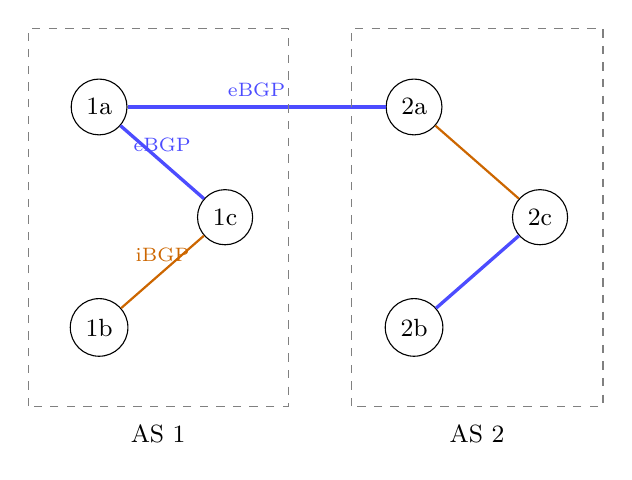
\begin{tikzpicture}[
    r/.style={circle, draw, minimum size=0.7cm, font=\small},
    lbl/.style={font=\small, align=center},
    e/.style={very thick, blue!70},
    i/.style={thick, orange!80!black}
]
    \node[r] (a1) at (0,1.4) {1a};
    \node[r] (a2) at (0,-1.4) {1b};
    \node[r] (a3) at (1.6,0) {1c};
    \draw[e] (a1)--(a3) node[midway, above, font=\scriptsize]{eBGP};
    \draw[i] (a2)--(a3) node[midway, above, font=\scriptsize]{iBGP};

    \node[r] (b1) at (4.0,1.4) {2a};
    \node[r] (b2) at (4.0,-1.4) {2b};
    \node[r] (b3) at (5.6,0) {2c};
    \draw[i] (b1)--(b3);
    \draw[e] (b2)--(b3);

    \draw[e] (a1) -- node[midway, above, font=\scriptsize]{eBGP} (b1);

    \draw[dashed, gray] (-0.9,-2.4) rectangle (2.4,2.4);
    \node[lbl] at (0.75,-2.75) {AS 1};
    \draw[dashed, gray] (3.2,-2.4) rectangle (6.4,2.4);
    \node[lbl] at (4.8,-2.75) {AS 2};
\end{tikzpicture}
\caption{eBGP 跨 AS 交换路由，iBGP 在 AS 内部分发（蓝色 eBGP，橙色 iBGP）}
\label{fig:bgp}
\end{figure}

\subsection{路径属性与选路决策}

BGP 通告携带多种\textbf{路径属性 (path attributes)}，它们是策略的载体：

\begin{table}[H]
\centering
\caption{BGP 常用路径属性}
\renewcommand{\arraystretch}{1.3}
\begin{tabulary}{\textwidth}{@{}CL@{}}
\toprule
\textbf{属性} & \textbf{含义} \\
\midrule
AS-PATH & 到达该前缀所经过的 AS 序列，用于环路检测与长度比较 \\
NEXT-HOP & 到达该前缀应交给的下一跳（边界路由器）地址 \\
LOCAL-PREF & 本地偏好，值越大越优先，用于表达「我更爱走这条出口」 \\
MED & 多出口鉴别器，向相邻 AS 建议入口偏好 \\
\bottomrule
\end{tabulary}
\end{table}

当同一前缀收到多条 BGP 路由时，路由器按以下（简化）顺序逐级比较，先满足者胜出：

\begin{enumerate}
    \item \textbf{本地偏好 LOCAL-PREF} 最高者优先（本地策略第一）；
    \item \textbf{AS 路径最短}：AS-PATH 中 AS 数最少；
    \item \textbf{热土豆路由 (hot potato routing)}：在仍打平的情况下，选择\textbf{本 AS 内到 NEXT-HOP 代价最小}（最近出口）的路由，尽快把分组「扔」出本 AS；
    \item 仍打平则用 BGP 标识符等做最终裁决。
\end{enumerate}

\textbf{热土豆路由}的直觉：本 AS 不关心分组出了本 AS 之后的命运，只求尽快、尽量省地把它交出去，代价就是 IGP 距离。它是典型的\textbf{策略路由}——最终路径未必是端到端最短，而是各 AS 各自决策的合成结果。

\section{ICMP：差错与控制报文}

IP 本身不可靠，也不报告错误。辅助它的是 \textbf{ICMP (Internet Control Message Protocol)}，它封装在 IP 数据报中（IPv4 协议号 1），用于传递差错与控制信息。ICMP 报文格式为：\textbf{类型 (type)} $+$ \textbf{代码 (code)} $+$ \textbf{检验和} $+$ 前 4 字节随类型而变 $+$ 可选数据区（通常携带触发该报文的原始 IP 首部及前 8 字节载荷，便于源端定位）。

\begin{table}[H]
\centering
\caption{常见 ICMP 报文类型}
\renewcommand{\arraystretch}{1.3}
\begin{tabulary}{\textwidth}{@{}CLC@{}}
\toprule
\textbf{类型} & \textbf{名称} & \textbf{典型用途} \\
\midrule
0 / 8 & 回显应答 / 回显请求 & \texttt{ping} 探测可达性与时延 \\
3 & 目的地不可达 & 网络/主机/端口不可达 \\
11 & 超时 & TTL 耗尽（\texttt{traceroute} 依赖） \\
5 & 重定向 & 提示更优的下一跳网关 \\
\bottomrule
\end{tabulary}
\end{table}

\subsection{\texttt{ping}}

若源主机周期性发送\textbf{回显请求 (type 8)}，目的主机回以\textbf{回显应答 (type 0)}。据此可测往返时间 (RTT) 与丢包率。注意许多主机会屏蔽 ICMP，因此「ping 不通」并不等价于「不可达」。

\subsection{\texttt{traceroute} 原理：TTL 递增}

\texttt{traceroute} 巧妙地利用 IP 首部的 \textbf{TTL} 字段与 ICMP 超时报文逐跳探测路径：

\begin{enumerate}
    \item 源主机依次发送一系列目的为同一目标、但 TTL $=1,2,3,\dots$ 的分组（通常用不可达的高端口 UDP 或 ICMP 回显请求）；
    \item TTL $=1$ 的分组到达第一跳路由器时 TTL 减为 $0$，被丢弃，路由器回送一个 \textbf{ICMP 超时 (type 11)} 报文，其中携带该路由器的地址；
    \item 源据此得知第 1 跳；随后 TTL $=2$ 的分组在第二跳耗尽，如此递推；
    \item 当分组终于到达目的主机时，目的端返回「端口不可达」(type 3, code 3) 或回显应答，探测结束。
\end{enumerate}

\begin{figure}[H]
\centering
\begin{tikzpicture}[
    h/.style={rectangle, draw, minimum width=1.0cm, minimum height=0.6cm, font=\small},
    arr/.style={-{Stealth[length=2.5mm]}, thick},
    lbl/.style={font=\scriptsize, align=center}
]
    \node[h] (s) at (0,0) {源};
    \node[h] (r1) at (2.6,0) {$R_1$};
    \node[h] (r2) at (5.2,0) {$R_2$};
    \node[h] (d) at (7.8,0) {目的};

    \draw[arr] (s.south) -- (r1.south) node[lbl, midway, below]{TTL$=1$ 耗尽};
    \draw[arr] (r1.north) to[bend left=40] node[lbl, above]{ICMP 超时} (s.north);
    \draw[arr] (s) -- (r2) node[lbl, midway, below, yshift=-1.4cm]{TTL$=2$};
    \draw[arr] (r2.north) to[bend left=55] node[lbl, above]{ICMP 超时} (s.north);
    \draw[arr] (s.south) to[bend right=8] (d.south) node[lbl, midway, below, yshift=-2.6cm]{TTL 足够大，到达目的};
    \draw[arr] (d.north) to[bend left=15] node[lbl, above]{端口不可达} (r2.north);
\end{tikzpicture}
\caption{\texttt{traceroute}：逐步增大 TTL，靠沿途 ICMP 超时报文勾出整条路径}
\label{fig:traceroute}
\end{figure}

\section{SDN：集中式控制平面}

传统路由器把控制平面（路由计算）和数据平面（转发）耦合在同一台设备内，每台各自运行分布式协议。\textbf{软件定义网络 (Software-Defined Networking, SDN)} 把二者解耦：控制平面集中到一台（或一簇）远程\textbf{控制器}，数据平面退化为通用、简单的\textbf{交换机}，只按控制器下发的规则做匹配与动作。

\subsection{OpenFlow：匹配$+$动作}

SDN 的南向接口以 \textbf{OpenFlow} 为代表。每台交换机的\textbf{流表 (flow table)} 由若干\textbf{流表项}组成，每项包含三部分：

\begin{itemize}
    \item \textbf{匹配字段 (match)}：对分组首部若干字段的匹配条件，可跨层组合，如入端口、源/目的 MAC、源/目的 IP、源/目的端口（TCP/UDP）、以及 VLAN、协议号等。支持通配（如 \texttt{10.0.0.*}）。
    \item \textbf{计数器 (counters)}：统计匹配到的分组数与字节数，供监控使用。
    \item \textbf{动作 (actions)}：匹配成功后执行的操作——\textbf{转发}到某端口、\textbf{丢弃}、\textbf{改写}（改 IP/端口）、或\textbf{送控制器}处理。
\end{itemize}

这一「\textbf{匹配$+$动作}」抽象统一了路由器、交换机、防火墙的功能：转发表、访问控制、NAT 都可用流表项表达。当分组与任何表项都不匹配时，交换机默认把它上送控制器，由控制器（全局视图下）决定下发新规则或直接处置。

\begin{table}[H]
\centering
\caption{OpenFlow 流表项示例}
\renewcommand{\arraystretch}{1.3}
\begin{tabulary}{\textwidth}{@{}LCC@{}}
\toprule
\textbf{匹配字段} & \textbf{动作} & \textbf{计数} \\
\midrule
入端口 $=1$, 目的 IP $=10.1.1.7$ & 转发端口 $3$ & 1240 包 \\
目的 IP $=10.2.0.0/16$ & 丢弃 & 87 包 \\
源 MAC $=\text{\texttt{00:..:A1}}$ & 送控制器 & 12 包 \\
\bottomrule
\end{tabulary}
\end{table}

\subsection{分层接口}

SDN 的架构常用三类接口描述：

\begin{itemize}
    \item \textbf{南向接口 (southbound)}：控制器 $\to$ 交换机，下发流表、查询状态，如 OpenFlow。
    \item \textbf{北向接口 (northbound)}：控制器 $\to$ 上层应用/编排系统，暴露抽象的网络视图与编程接口（如 REST）。路由、负载均衡、防火墙等应用在其上编程，而无需接触底层设备。
    \item \textbf{东向/西向接口}：多个控制器之间的横向通信，用于大规模网络下的控制平面扩展与一致。
\end{itemize}

\begin{figure}[H]
\centering
\begin{tikzpicture}[
    box/.style={draw, rounded corners, minimum width=2.1cm, minimum height=0.7cm, font=\small, align=center},
    arr/.style={{Stealth[length=2.5mm]}-{Stealth[length=2.5mm]}, thick}
]
    \node[box, fill=green!15] (app) at (0,2.6) {网络应用\\（路由/防火墙）};
    \node[box, fill=blue!15, minimum width=3.0cm] (ctrl) at (0,1.1) {SDN 控制器};
    \node[box] (s1) at (-3.2,-0.7) {交换机 1};
    \node[box] (s2) at (0,-0.7) {交换机 2};
    \node[box] (s3) at (3.2,-0.7) {交换机 3};

    \draw[arr] (app) -- (ctrl) node[midway, right, font=\scriptsize]{北向接口};
    \draw[arr] (ctrl) -- (s1) node[midway, left, font=\scriptsize]{南向};
    \draw[arr] (ctrl) -- (s2) node[midway, right, font=\scriptsize]{南向接口};
    \draw[arr] (ctrl) -- (s3) node[midway, right, font=\scriptsize]{南向};
\end{tikzpicture}
\caption{SDN 分层：应用经北向接口编程，控制器经南向接口（OpenFlow）下发流表}
\label{fig:sdn}
\end{figure}

\section{本章小结与常见误区}

\noindent\textbf{知识主线}：控制平面由\textbf{路由算法}计算转发表。\textbf{链路状态}算法让每个节点获得全网图，再用 \textbf{Dijkstra} 求最短路，工程化为 \textbf{OSPF}；\textbf{距离向量}算法让节点与邻居迭代交换向量，基于 \textbf{Bellman--Ford} 方程，典型协议是 RIP，其固有弱点是\textbf{计数到无穷}，需靠水平分割/毒性逆转缓解。跨 AS 的路由由 \textbf{BGP} 承担，它是\textbf{路径向量}协议，强调\textbf{策略}而非最短，eBGP 跨域、iBGP 域内传播。\textbf{ICMP} 承载差错与控制报文，是 \texttt{ping} 与 \texttt{traceroute} 的基础。\textbf{SDN} 把控制平面集中到控制器，用 OpenFlow 的「匹配$+$动作」流表统一转发。

常见误区：

\begin{itemize}
    \item \textbf{「路由算法一定求最短路径」}：BGP 的目标是策略与可达性，最终路径常常并非端到端最短；热土豆路由就是「只求尽快出本 AS」。
    \item \textbf{「Dijkstra 的 $D(v)$ 就是最终最短路」}：在被选入 $N'$ 之前，$D(v)$ 只是上界估计；只有加入 $N'$ 时才确定。
    \item \textbf{「DV 一定能收敛到正确值」}：坏消息下可能出现计数到无穷；若网络无直连替代路径且无缓解机制，估计值会无限增大。
    \item \textbf{「毒性逆转能彻底解决环路」}：它只切断两节点环路，长度 $\ge 3$ 的环路仍可能存在。
    \item \textbf{「iBGP 是另一种协议」}：iBGP 与 eBGP 同属 BGP，区别只在会话两端是否处于同一 AS。
    \item \textbf{「ping 不通说明主机离线」}：ICMP 常被防火墙屏蔽，「不通」只说明没有回显应答。
    \item \textbf{「SDN 就是 OpenFlow」}：OpenFlow 只是主流南向协议之一；SDN 的本质是控制平面与数据平面\textbf{解耦}与集中控制。
    \item \textbf{「链路状态泛洪没有代价」}：泛洪是 $O(|E|)$ 量级的全网开销，OSPF 的分区域正是为限制它。
\end{itemize}
